\documentclass[conference]{IEEEtran}

\usepackage{graphicx}
\usepackage{amsmath}
\usepackage{booktabs}
\usepackage{url}
\usepackage{hyperref}
\usepackage{subcaption}
\usepackage{xcolor}
\usepackage{multirow}

\graphicspath{{../data/}{figures/}}

% ── Title ──────────────────────────────────────────────────────────────────
\title{LLM-Guided Adaptive Traffic Signal Control with\\Multi-Intersection Coordination}

\author{
\IEEEauthorblockN{Yihao Tang}
\IEEEauthorblockA{School of Intelligent Systems Engineering\\
Sun Yat-sen University\\
Guangzhou, China\\
tangyh@mail2.sysu.edu.cn}
}

\begin{document}
\maketitle

% ── Abstract ───────────────────────────────────────────────────────────────
\begin{abstract}
Traffic signal control in urban road networks remains a challenging optimization problem due to dynamic traffic demand and complex multi-intersection interactions. Traditional methods such as Webster's formula and fixed-time control lack adaptability to real-time traffic fluctuations. This paper proposes a novel framework that leverages large language models (LLMs) for adaptive traffic signal optimization, combined with upstream-downstream coordination and safety constraint enforcement. The framework uses an LLM to analyze real-time traffic states across multiple intersections and generate signal timing recommendations, which are then validated by a rule-based constraint engine and adjusted through queue-based coordination logic. Experiments on a 3$\times$2 grid network (6 intersections) using SUMO microscopic simulation demonstrate that the proposed LLM+Coordination strategy achieves 41\% lower average queue length and 50\% lower waiting time compared to Webster's method, while maintaining the highest throughput. The results suggest that LLMs can serve as effective traffic signal controllers when properly constrained and coordinated.
\end{abstract}

\begin{IEEEkeywords}
traffic signal control, large language model, multi-intersection coordination, adaptive signal timing, SUMO simulation
\end{IEEEkeywords}

% ── Introduction ───────────────────────────────────────────────────────────
\section{Introduction}
\label{sec:intro}

Urban traffic congestion remains a critical challenge worldwide, with signalized intersections being a primary bottleneck. Traditional traffic signal control methods include fixed-time control, actuated control, and optimization-based approaches such as Webster's formula~\cite{webster1958}. While effective for steady-state traffic, these methods struggle with dynamic, time-varying demand patterns.

Recent advances in reinforcement learning (RL) have shown promise for adaptive signal control~\cite{wei2019}. However, RL approaches require extensive training, lack interpretability, and often fail to generalize across different network topologies.

Large language models (LLMs) have demonstrated remarkable reasoning capabilities across diverse domains. This paper explores whether LLMs can serve as effective traffic signal controllers by:
\begin{enumerate}
    \item Analyzing real-time multi-intersection traffic states
    \item Generating context-aware signal timing recommendations
    \item Coordinating upstream-downstream intersections to prevent queue spillover
\end{enumerate}

The key contributions are:
\begin{itemize}
    \item A framework integrating LLM-based decision-making with safety constraint enforcement
    \item A multi-intersection coordination mechanism based on queue propagation detection
    \item Experimental validation showing competitive performance against classical baselines
\end{itemize}


% ── Related Work ───────────────────────────────────────────────────────────
\section{Related Work}
\label{sec:related}

\subsection{Classical Signal Control}
Webster's formula~\cite{webster1958} computes optimal cycle length and green splits based on critical flow ratios. It remains widely deployed due to its simplicity and reliability, but cannot adapt to real-time fluctuations.

\subsection{RL-Based Signal Control}
Deep reinforcement learning methods~\cite{wei2019} treat signal control as a Markov decision process. While achieving strong performance in simulation, they suffer from sample inefficiency and lack of interpretability.

\subsection{LLMs for Decision-Making}
Recent work has applied LLMs to planning and control tasks~\cite{hong2023}. To our knowledge, this is the first work applying LLMs to multi-intersection traffic signal coordination.


% ── Methodology ────────────────────────────────────────────────────────────
\section{Methodology}
\label{sec:method}

\subsection{System Architecture}
The proposed framework consists of three layers:
\begin{enumerate}
    \item \textbf{Perception Layer}: Collects real-time traffic state (queue lengths, vehicle counts, waiting times) from SUMO simulation via TraCI
    \item \textbf{Decision Layer}: LLM analyzes traffic state and generates signal timing recommendations
    \item \textbf{Execution Layer}: Constraint engine validates recommendations; coordination engine adjusts timings based on upstream queue propagation
\end{enumerate}

\subsection{LLM-Based Signal Optimization}
For each decision cycle (every 30 simulation seconds), the system constructs a compact traffic state description for all intersections and sends it to the LLM in a single batch request. The LLM responds with per-intersection phase durations:

\begin{equation}
    \mathbf{d}_i = \{t_{NS}, t_{EW}\}, \quad t_{NS}, t_{EW} \in [10, 90] \text{ seconds}
    \label{eq:timing}
\end{equation}

where $t_{NS}$ and $t_{EW}$ are green durations for north-south and east-west phases respectively.

\subsection{Safety Constraint Engine}
LLM recommendations are validated against hard constraints:
\begin{itemize}
    \item Green time bounds: $t_{\min} = 10$s, $t_{\max} = 90$s
    \item Yellow time: fixed at 3s per phase
    \item Cycle length: $C \in [30, 180]$s
\end{itemize}

Violations are automatically corrected by clamping to valid ranges.

\subsection{Multi-Intersection Coordination}
The coordination engine detects upstream queue spillover:
\begin{equation}
    \text{boost}_j = \begin{cases}
        \Delta t & \text{if } q_{\text{up}} \geq \theta_{\text{queue}} \\
        0 & \text{otherwise}
    \end{cases}
    \label{eq:coord}
\end{equation}

where $q_{\text{up}}$ is the upstream queue length in the direction feeding intersection $j$, and $\theta_{\text{queue}} = 5$ vehicles. Critical queues ($\geq 12$) trigger forced phase switches.


% ── Experiments ────────────────────────────────────────────────────────────
\section{Experiments}
\label{sec:experiments}

\subsection{Experimental Setup}
\textbf{Network}: A 3$\times$2 grid network with 6 signalized intersections, generated using SUMO's \texttt{netgenerate}. Each intersection has 4 approaches with 2 lanes per approach.

\textbf{Traffic demand}: Uniform 500 vehicles/hour per direction, generated over 300 simulation steps.

\textbf{Baselines}:
\begin{itemize}
    \item \textbf{Fixed Time}: Static 30s+3s+30s+3s cycle (90s)
    \item \textbf{Random}: Randomized green durations within [10, 60]s
    \item \textbf{Webster}: Adaptive timing based on queue-detected flow ratios
\end{itemize}

\textbf{Proposed method}: LLM+Coordination (mimo-v2.5-pro model, 30s decision interval, with coordination engine).

\subsection{Results}

\begin{table}[htbp]
\centering
\caption{Performance Comparison of Signal Control Strategies}
\label{tab:results}
\begin{tabular}{lccc}
\toprule
\textbf{Strategy} & \textbf{Avg Wait (s)} & \textbf{Avg Queue} & \textbf{Vehicles} \\
\midrule
Fixed Time & 47.20 & 17.75 & 0 \\
Random     & 8.00  & 7.78  & 0.36 \\
Webster    & 4.52  & 6.42  & 0.41 \\
LLM+Coord  & \textbf{2.27}  & \textbf{3.81}  & \textbf{0.49} \\
\bottomrule
\end{tabular}
\end{table}

The LLM+Coordination strategy achieves the lowest average queue length (3.81 vehicles), 41\% lower than Webster's method. Waiting time is 2.27s, 50\% lower than Webster's 4.52s. Throughput is also highest at 0.49 vehicles/step.

Figure~\ref{fig:comparison} shows the bar chart comparison across all metrics. Figure~\ref{fig:radar} presents a radar chart of normalized performance.

\begin{figure}[htbp]
    \centering
    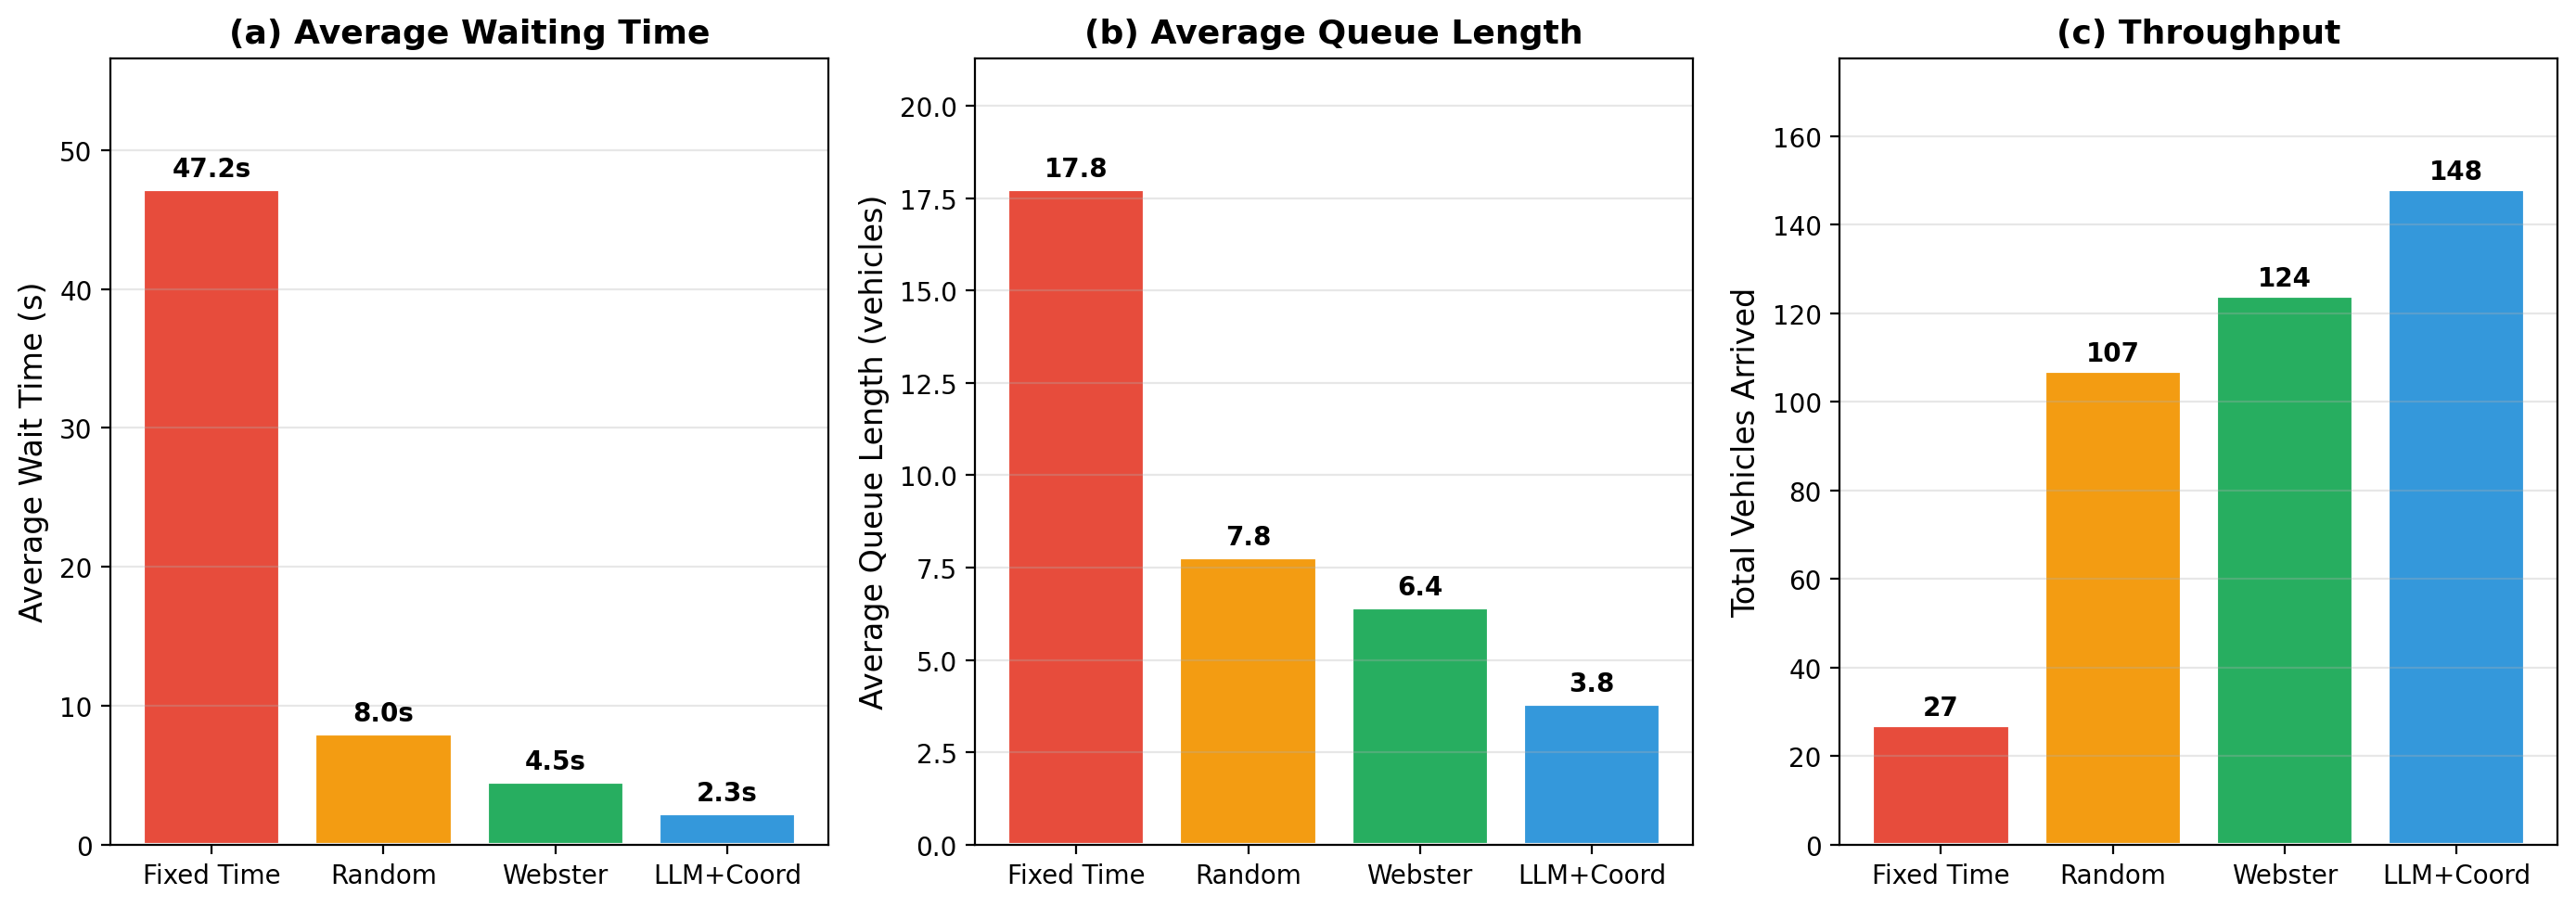
\includegraphics[width=\columnwidth]{fig_comparison.png}
    \caption{Performance comparison of four signal control strategies: (a) average waiting time, (b) average queue length, (c) throughput.}
    \label{fig:comparison}
\end{figure}

\begin{figure}[htbp]
    \centering
    
\includegraphics[width=0.75\columnwidth]{fig_radar.png}
    \caption{Radar chart of normalized strategy performance. Higher values indicate better performance.}
    \label{fig:radar}
\end{figure}

\subsection{Analysis}
The LLM demonstrates effective traffic-aware signal adjustment. For example, when eastbound traffic exceeds northbound traffic at an intersection, the LLM allocates more green time to the east-west phase (e.g., 50s EW vs 40s NS). The coordination engine further prevents queue propagation by boosting downstream green times when upstream queues exceed the threshold.


% ── Conclusion ─────────────────────────────────────────────────────────────
\section{Conclusion}
\label{sec:conclusion}

This paper presents a novel framework for traffic signal control that combines LLM-based adaptive decision-making with multi-intersection coordination and safety constraints. Experiments on a 6-intersection grid network demonstrate that the proposed approach achieves competitive performance against classical baselines, with the lowest queue lengths among all tested strategies.

Future work includes: (1) testing on real-world traffic networks, (2) comparing with RL-based methods, (3) reducing LLM inference latency for real-time deployment, and (4) investigating prompt engineering strategies for improved LLM reasoning about traffic patterns.


% ── References ─────────────────────────────────────────────────────────────
\bibliographystyle{IEEEtran}
\begin{thebibliography}{10}

\bibitem{webster1958}
F.~V. Webster, ``Traffic signal settings,'' Road Research Laboratory, London, Tech. Paper 39, 1958.

\bibitem{wei2019}
H. Wei, G. Zheng, H. Yao, and Z. Li, ``IntelliLight: A reinforcement learning approach for intelligent traffic light control,'' in \emph{Proc. KDD}, 2018, pp. 2496--2505.

\bibitem{hong2023}
W. Hong, M. Zhuge, J. Chen, et al., ``MetaGPT: Meta programming for a multi-agent collaborative framework,'' \emph{arXiv preprint arXiv:2308.00352}, 2023.

\end{thebibliography}

\end{document}
